\documentclass{article}
\usepackage{amsthm, amsmath, listings, graphicx}
\usepackage[margin=0.5in]{geometry}
\graphicspath{ {hw4_img/} }

\begin{document}
\noindent\textbf{CS 375 Homework 4}\hfill Anchu A. Lee\\
\noindent\today
\\\\“I have done this assignment completely on my own. I have not copied it, nor have I given my solution to anyone else. I understand that if I am involved in plagiarism or cheating I will have to sign an official form that I have cheated and that this form will be stored in my official university record. I also understand that I will receive a grade of 0 for the involved assignment for my first offense and that I will receive a grade of “F” for the course for any additional offense.” 
\\\\
\begin{enumerate}
    \item A set $\{3, 4, 5, 8\}$ is given. For the set, find \textbf{every 
    subset} that sums to $S = 13$. Find the subsets via the backtracking 
    algorithm. In your solution, draw a pruned state space tree. For each node 
    in the tree, show its current subset sum and its upper bound of the sum 
    (i.e., $weightSoFar + totalPossibleLeft$). Number the nodes in the 
    sequence of visiting them. Also, identify the node that represents the 
    solution found at the end of the search.\newline
    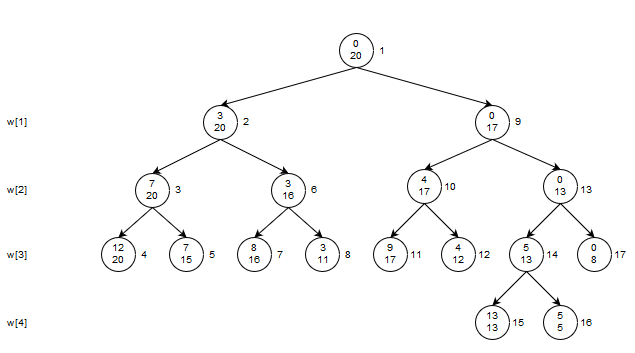
\includegraphics[scale=0.8]{p1_tree}
    \item When the capacity of the knapsack is 15, solve the following 
    \textbf{0-1 knapsack} problem using the backtracking algorithm that uses 
    the optimal fractional knapsack algorithm to compute the upper bound of 
    the profit.\newline
    \begin{tabular}{c c c c}
        $i$ & $p_i$ & $w_i$ & $p_i / w_i$\\
        1 & \$10 & 5 & \$2\\
        2 & \$30 & 2 & \$15\\
        3 & \$40 & 5 & \$8\\
        4 & \$30 & 10 & \$3
    \end{tabular}\newline
    In your solution, draw a pruned state space tree. For each node in the 
    tree, show its profit, weight, and upper bound of the profit. Number the 
    nodes in the sequence of visiting them. Also, identify the node that 
    represents the optimal solution found at the end of the search.\newline
    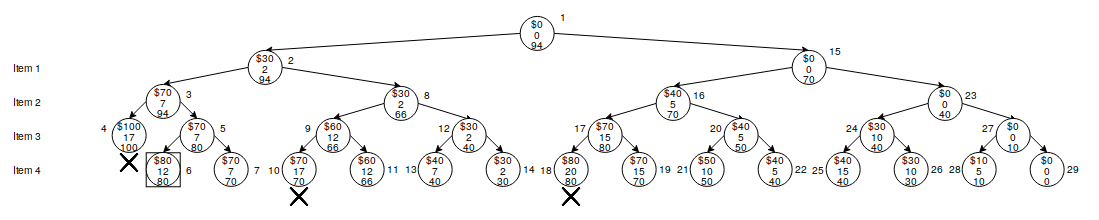
\includegraphics[scale=0.48]{p2_tree}

    \item For the same problem in Question 2, solve it using the best-first-
    search branch and bound algorithm. Follow the same instructions above to 
    produce your solution.\newline
    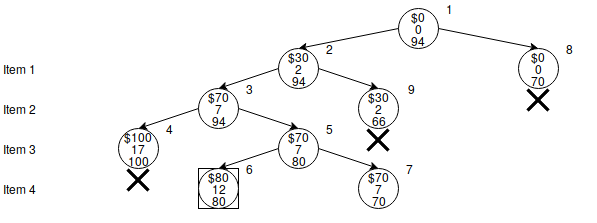
\includegraphics[scale=0.6]{p3_tree}
    
    \item Apply Prim's algorithm for finding a minimum spanning tree for the 
    following graph. Start with node a. Show the steps by filling out the 
    following table (see the example on slide 31 of lecture 25). Show the 
    selected tree nodes in the first column of the table, for each of the rest 
    of the nodes, show its minimum distance $D$ to the current tree and its 
    nearest node in the current tree, in the remaining columns.\newline
    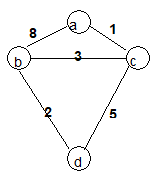
\includegraphics[scale=0.75]{p4_graph}\newline
    \begin{tabular}{|c |c |c |c |c|}
        \hline
        Node added to the current tree & $D(a)$, nearest node & $D(b)$, 
        nearest node & $D(c)$, nearest node & $D(d)$, nearest node\\
        \hline
        & & & &\\
        \hline
        & & & &\\
        \hline
        & & & &\\
        \hline
        & & & &\\
        \hline
    \end{tabular}
    
    \item Apply Kruskal’s algorithm for finding a minimum spanning tree for 
    the following graph. In your solution, show edges picked in order and the 
    total weight of the final minimum spanning tree.\newline
    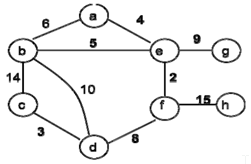
\includegraphics[scale=0.75]{p5_graph}\newline

    \item Using Dijkstra’s algorithm, find the shortest path to visit each 
    vertex starting from vertex s in the following graph. In your solution, 
    order the vertexes in terms of their shortest path distances to the vertex 
    s, and show the shortest path and its distance for each vertex. \newline
    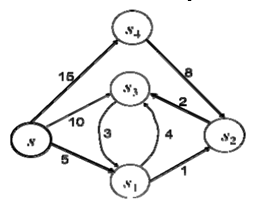
\includegraphics[scale=0.75]{p6_graph}\newline

    \item Apply Floyd-Warshall algorithm to the following directed graph with 
    the initial distance matrix representing the direct distance between every 
    pair of vertices, and produce the updated distance matrices for every 
    iteration of the algorithm. \newline
    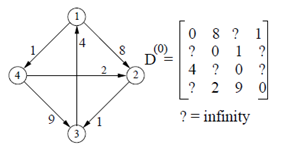
\includegraphics[scale=0.75]{p7_graph}\newline
\end{enumerate}
\end{document}